%\documentclass[a4paper,12pt,oneside,draft]{article}
\documentclass[a4paper,12pt,oneside]{article}

% In the original writelatex tamplate
\usepackage[english]{babel}
\usepackage[utf8]{inputenc}
\usepackage{amsmath}
\usepackage{graphics}
\usepackage[colorinlistoftodos]{todonotes}

% By LoCigno
\usepackage{times}
\usepackage{graphicx}
\usepackage{subfigure}
\usepackage{csvsimple}
\usepackage{color}
\usepackage{url}
\usepackage{hyperref} 
\usepackage{cleveref}

% By Davide
\usepackage{comment}
\usepackage{booktabs}
\usepackage{color}

%Variables macros
\newcommand{\DefineVar}[2]{%
  \expandafter\newcommand\csname var-#1\endcsname{#2}%
} 
\newcommand{\var}[1]{\csname var-#1\endcsname}

\usepackage{courier}
\newcommand{\mono}[1]{\texttt{#1}}

\title{Controller design for Lego Mindstorm motor}

\author{Diego Verona, Aliaksandr Siarohin, Mattia Digilio}

\date{\today}

% By Diego
\newtheorem{thm}[equation]{Theorem}
\usepackage[outdir=./]{epstopdf}
\usepackage{float}

\begin{document}
%\maketitle
\makeatletter  % populates \@title, \@author, \@date
\begin{titlepage}
      \centering
      ~~~~~~~~~~~~~\\[-30mm]
      
\includegraphics[keepaspectratio=true, width=7cm]{bg_eng_1r.jpg} \\[10mm]

     {
     \large \bfseries Master Degree in Computer Science\\[3mm] 
     Applied Robotics\\[3mm]
     AA 2015-2016
     }\\[10mm]

     %--------------------------------
     % Set the title, author, and date
     % 

     \vspace{0.5cm}
     {
     \Large \bfseries \textcolor{blue}{\@title} \par
     }
     \vspace{0.5cm}
%      {
%      \large {Group N. 1} \par
%      }
     \vspace{0.2cm}

     {\large {\@author}}
     \\ \vspace{.2cm}
     \@date

     \vspace{0.6cm}

    %-----------------------------------

\begin{abstract}

\textit{
  Report for the third assignment on Applied robotics: design and implement a simple model of vehicle that can go straight without additional sensors for the Lego NXT.\\In this report we show model of a vehicle, describing its properties and its digital implementation.
}


\end{abstract}

\end{titlepage}

\section{General definition}
\begin{thm}
\textbf{Root locus}. The \texttt{root locus}, or \texttt{Evans locus}, is a graphical method that
depicts the curves of the roots of the denominator of the closed loop transfer function in the complex plane
(sometimes called Argand plane or Gauss plane). The curves are parametrized by a parameter, typically the
gain of the loop.  \footnote{\url{http://disi.unitn.it/~palopoli/courses/ECL/RootLocus.pdf}}
\end{thm}
\begin{thm}
\textbf{Closed-loop transfer function}. A closed-loop transfer function in control theory is a mathematical expression (algorithm) describing the net result of the effects of a closed (feedback) loop on the input signal to the circuits enclosed by the loop. \footnote{\url{https://en.wikipedia.org/wiki/Closed-loop_transfer_function}}
\end{thm}

\section{Design of vehicle}
In this section is explained how the vehicle has been designed.
\subsection{Vehicle requirements}
The vehicle have to go straight without additional sensors and human interaction and to change its velocity according to the covered distance. The model of the robot needs at least three wheels and two motors: one wheel is free to move, others are controlled by the motors.
\subsection{Lego structure}
The structure of our Lego robot is shown in the pictures \cref{fig:back}, \cref{fig:front} and \cref{fig:left}. Distance between the driving wheels is $\approx$ 13cm and the radius of each wheel is $\approx$ 2.8 cm. 
\subsection{Controller design}
Each motor needs its own controller - called "inner controller" - and the direction of the vehicle is adjusted by an other controller called "outer controller". The overall structure can be found in: \cref{fig:diagram}.
\begin{figure}[h]
	\centering
	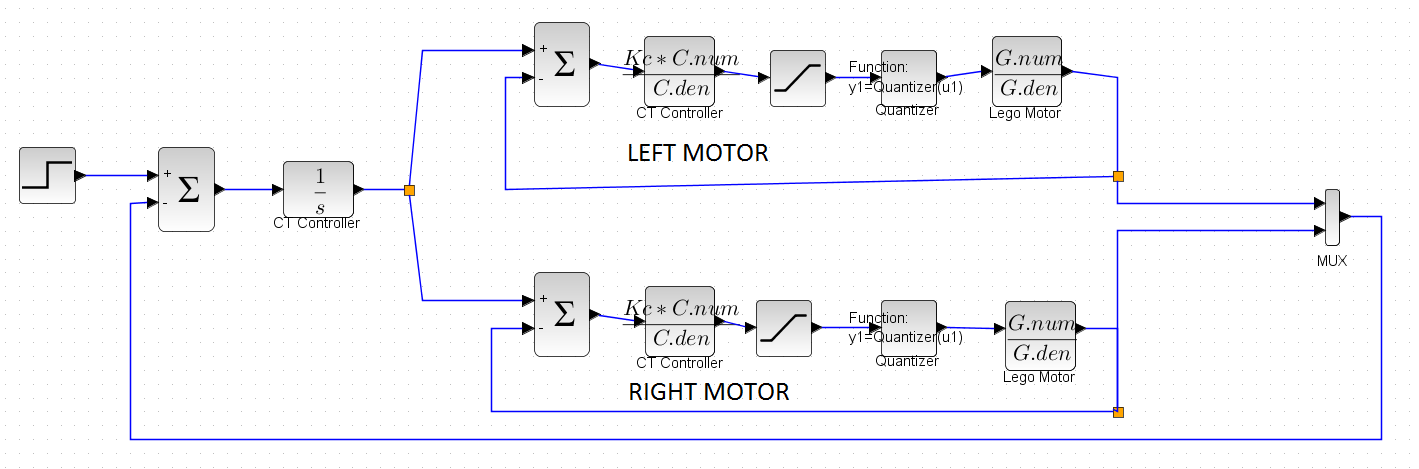
\includegraphics[width=\columnwidth]{vehicle.png}
	\caption{Structure of vehicle controller}
	\label{fig:diagram}
\end{figure}
\paragraph{Inner controllers}
About the inner controller refer to the second assignment of this course available on \url{https://github.com/AliaksandrSiarohin/AppliedRobotics/blob/master/report/lab2.pdf}.\\
\paragraph{Outer controller}
Outer controller need data from both motors and then it compute velocity and direction of the vehicle.\\
Velocity of the vehicle:
\begin{equation}
\text{velocity} = R \frac{velocity_A + velocity_B}{2} 
\end{equation}

Where R - is radius of the wheel. And $velocity_A$, $velocity_B$ is angular velocity of the motors. 

And the direction of the vehicle is:
\begin{equation}
\text{direction} = R \frac{velocity_B - velocity_A}{L}
\end{equation}

Where L is the distance between wheels. The direction should be 0 in order for vehicle to move straight.


\subsection{Controller implementation}
The main task is called every 5 ms and do this operations:
\begin{enumerate}
\item Compute current velocities of both motors using exponential average (as what has done on the assignment 2)
\item Compute vehicle velocity and direction. It has been setted that the vehicle has to travel for 3 meters: the first one with speed 3 rad/s, the second one with 6 rad/s and the last one with 9 rad/s. After that, the vehicle has to stop and stay there.
\item Adjust motors power based on inner and outer controllers.
\end{enumerate}

The entire implementation is downloadable from this Github folder: \url{https://github.com/AliaksandrSiarohin/AppliedRobotics/tree/master/motor_controller}
\section{Conclusion}

This third assignment is the conclusion of the course and the bases to farther projects. Starting from the theory applied and studied on simulations is it possible to apply it to the reality and obtain the wanted results. Thanks to this course has been possible to make realizable a simple idea in different ways and choose which one fit more between wanted and obtained results. Some chooses that has been done, for instances, were the best channel to getting data on assignment 1, the best parameters about root locus on assignment 2 and the physical errors of Logo structure this last assignment.\\ Also if our code is well done, simulation demonstrate that it has to work and the Lego structure is simple, solid and stable, the vehicle doesn't go perfectly straight because there are some implicit errors that can not be adjust with this simple system. This is not an ending point, but it is a good point to continue the study about physical limits, study better the environmental and all the external factors that influence the vehicle and add more sensor and complexity to the entire system.
\begin{figure}
	\centering
	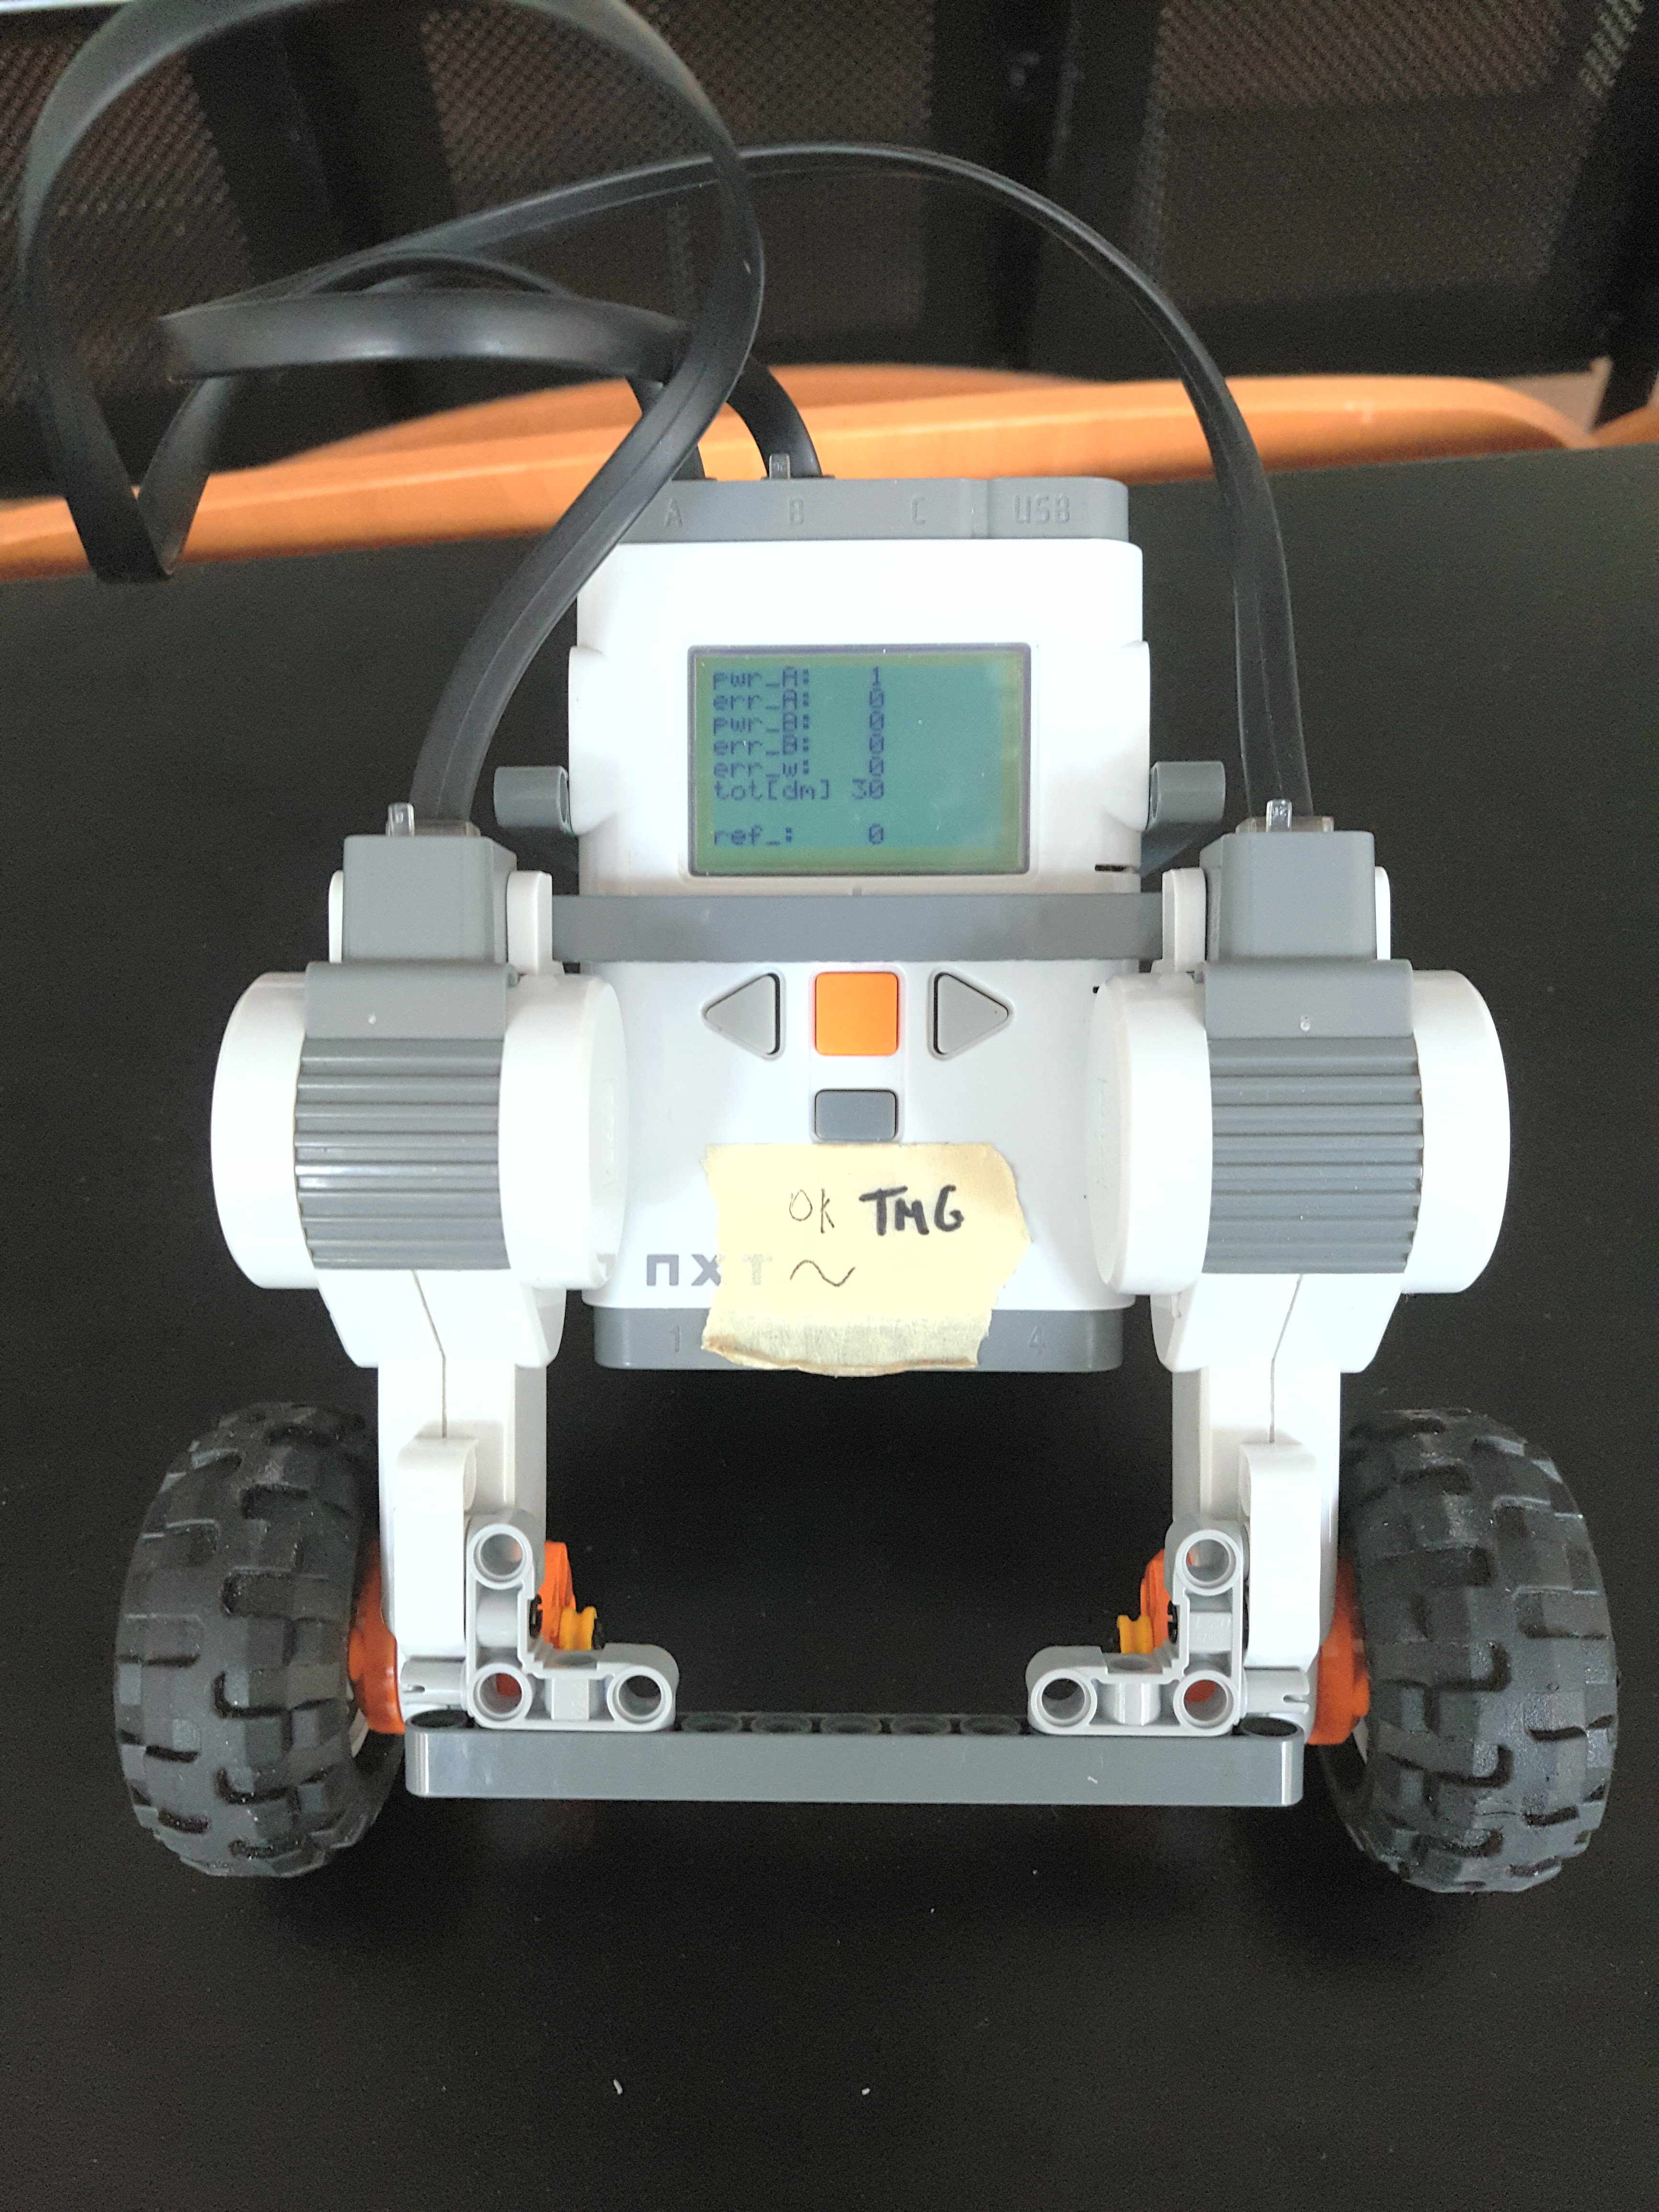
\includegraphics[width=\columnwidth]{nxtImages/1.jpg}
	\caption{Back side}
	\label{fig:back}
\end{figure}
\begin{figure}
	\centering
	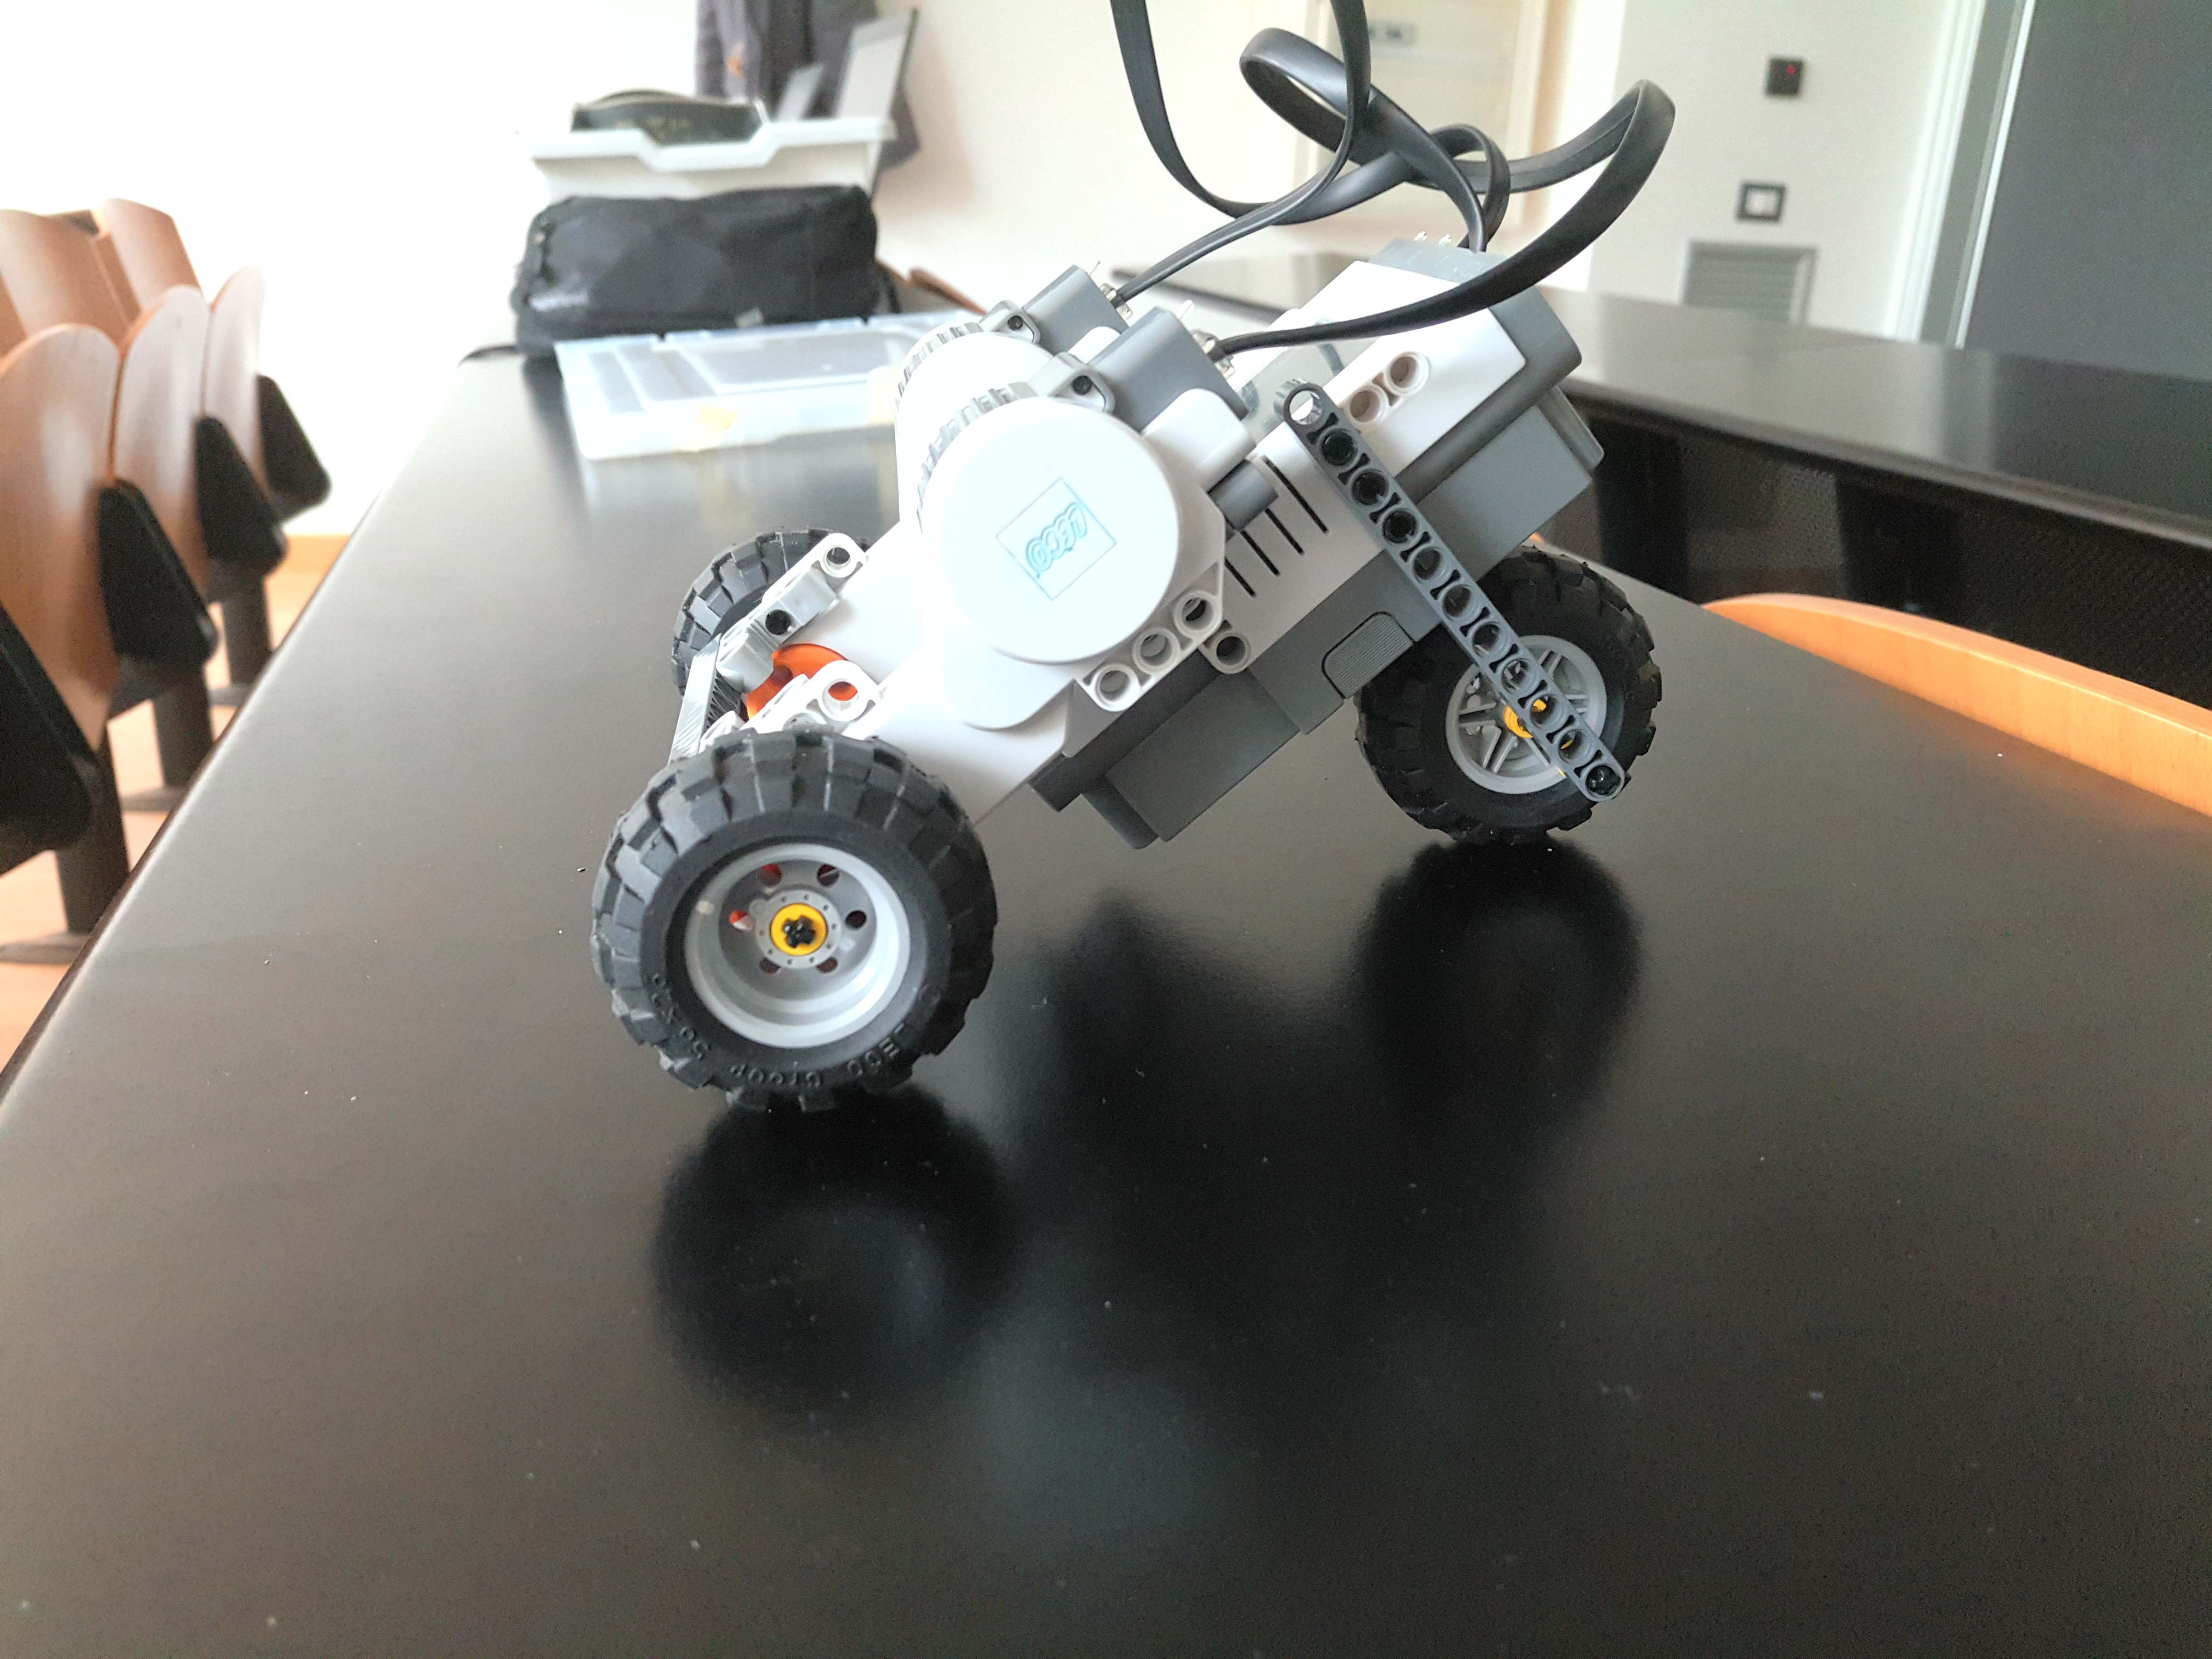
\includegraphics[width=\columnwidth]{nxtImages/2.jpg}
	\caption{Left side}
	\label{fig:left}
\end{figure}
\begin{figure}
	\centering
	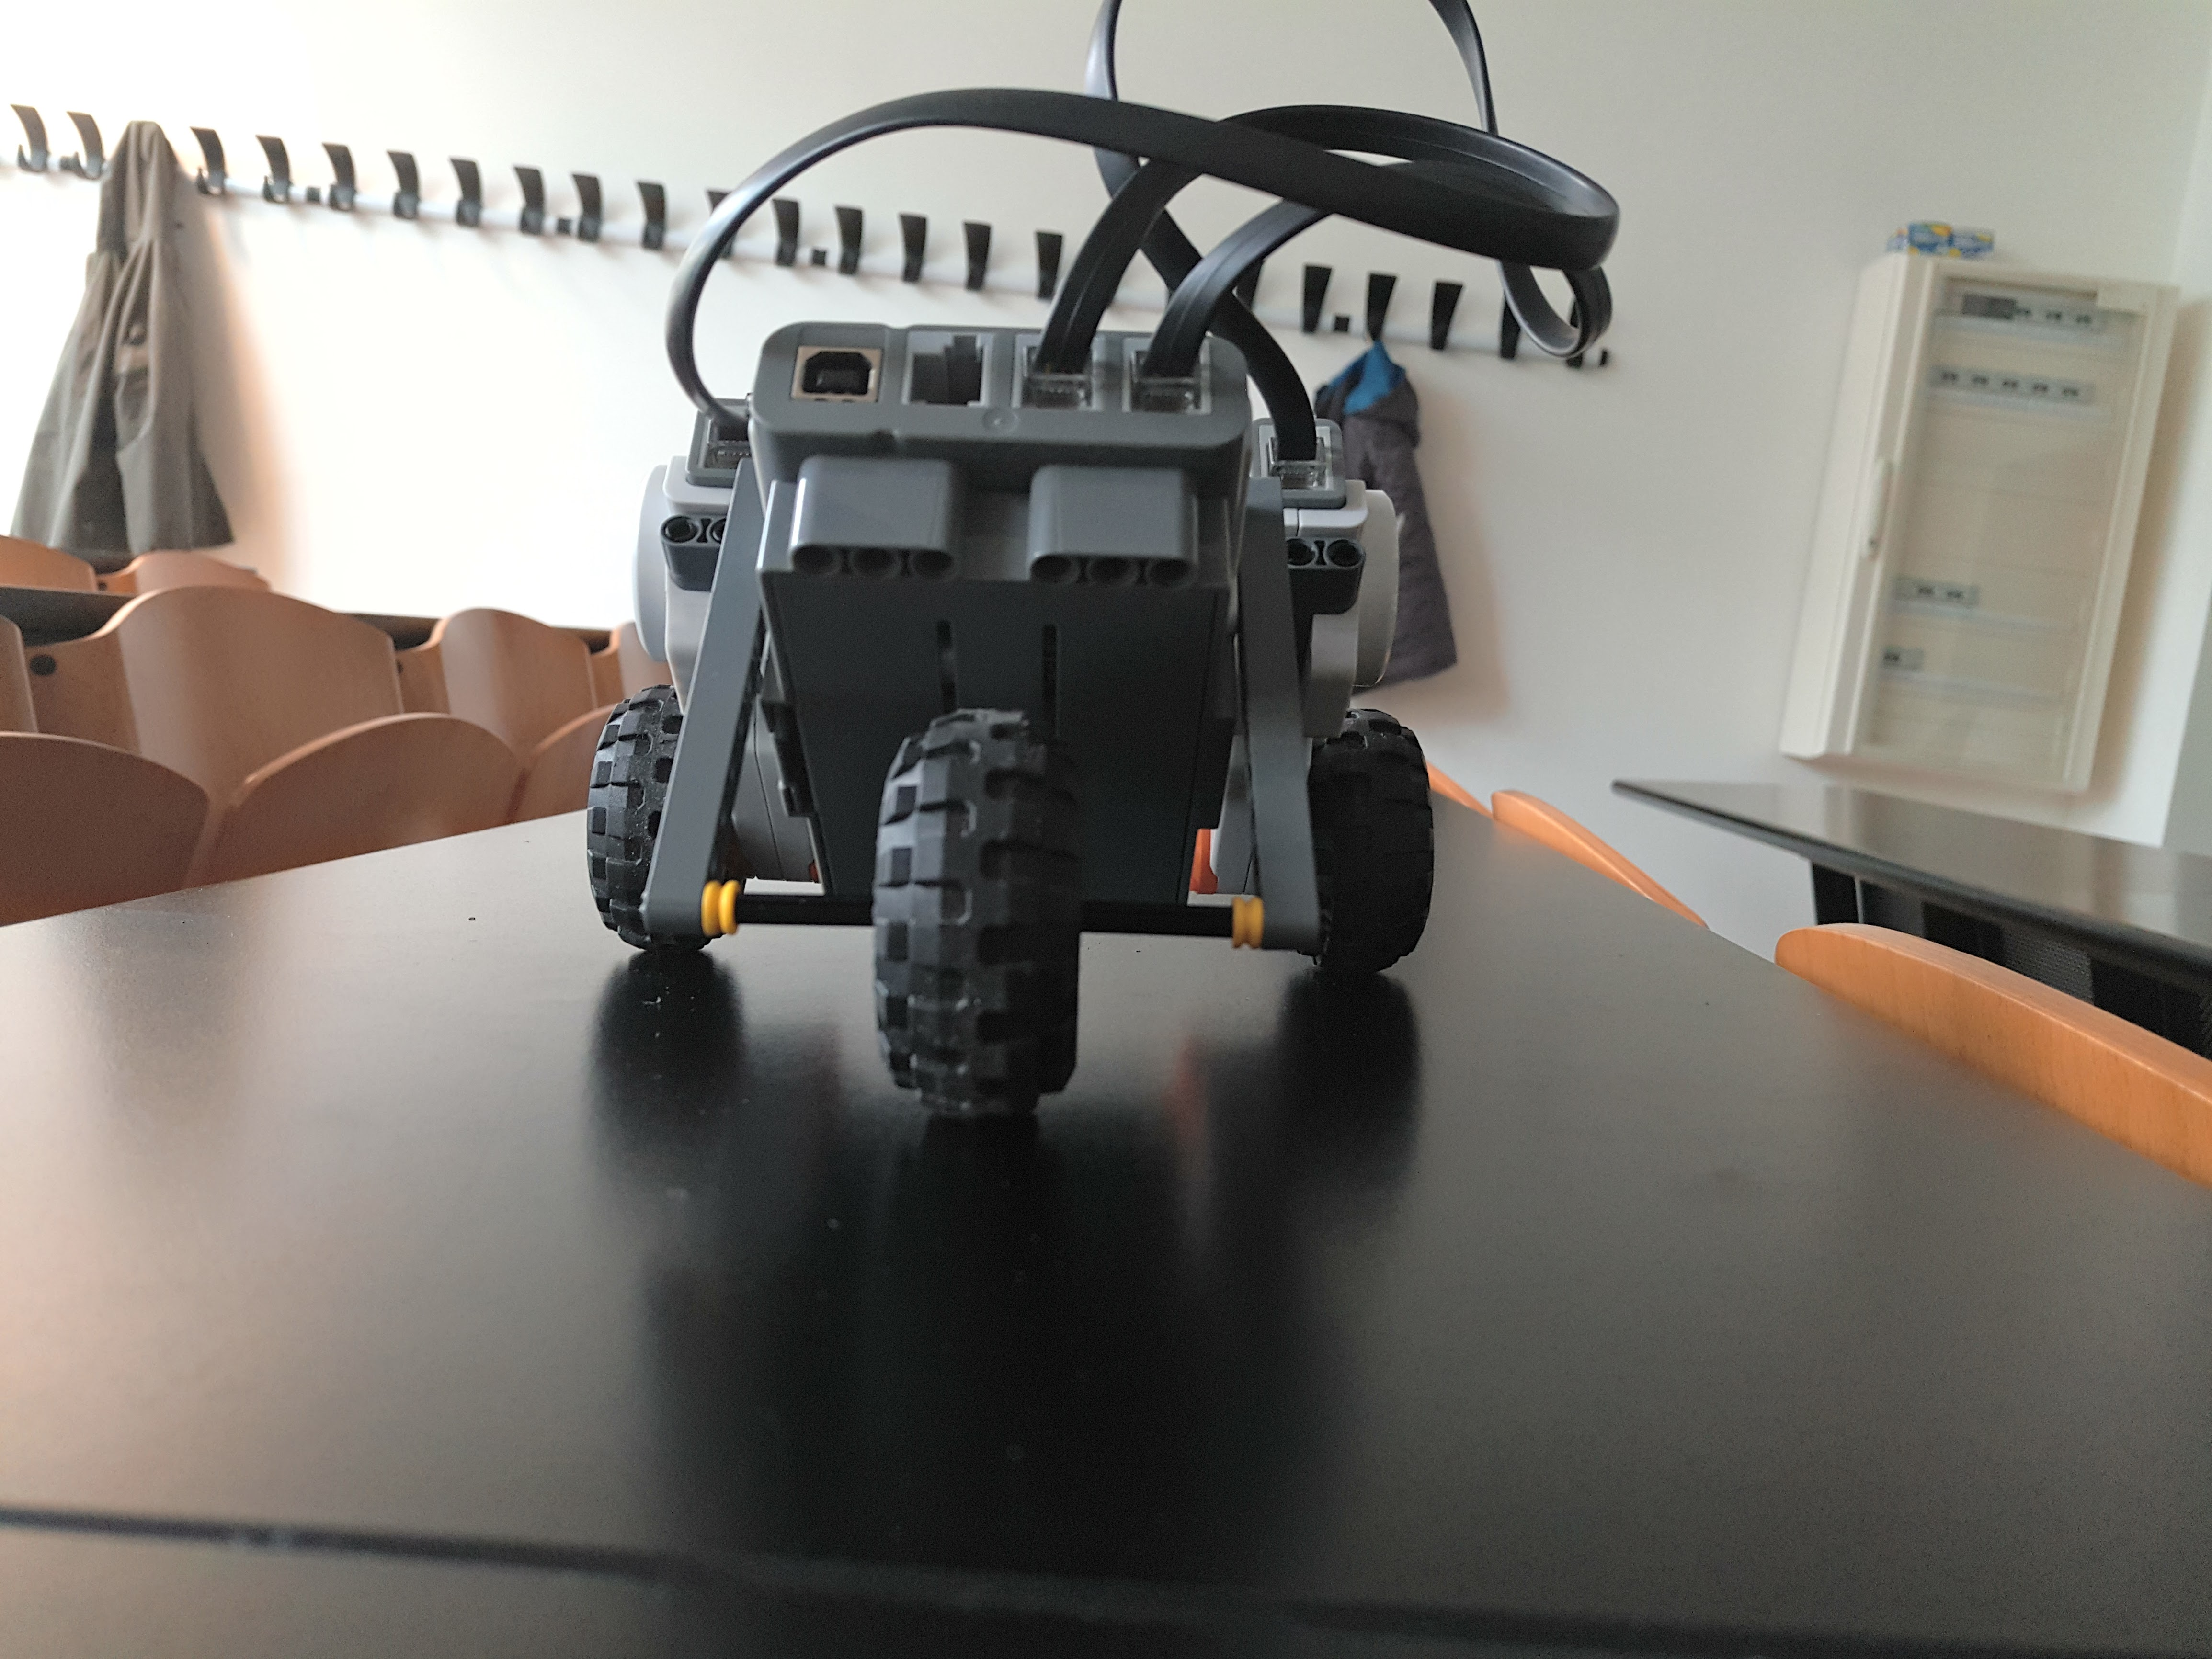
\includegraphics[width=\columnwidth]{nxtImages/3.jpg}
	\caption{Front side}
	\label{fig:front}
\end{figure}


\end{document}